\chapter{Deep Networks}\label{deepNets}
\chapterauthor{Jeff Yoshimi}

% Other topics: pooling, strides, or padding (mention in footnote)
% Discuss engineering, connectionism, CCN, and comp neuro. Maybe make that a final section
% Discuss deep fakes and GANs

The idea of re-mapping an input space to a hidden unit space in order to solve classification and regression problems is what drew neural networks out of its first ``dark age'' and back into the limelight, giving rise to an explosion of interest in engineering and connectionism in the 1980s and 1990s (chapter \extref{ch_history}). The internal representations of these networks--usually 3 layer networks trained by backprop--allowed them to solve previously unsolvable problems like XOR. They also developed psychologically realistic internal representations. However, recall that a second  winter lay in wait, as machine learning models took over in the late 1990s and 2000s. What got us out of that second winter was \glossary{deep network}s, that is, networks with more than 3 node layers, trained using new tricks and techniques, like convolutional layers, the use of graphical processing units for fast parallel computation, and the Relu activation function discussed in chapter \extref{ch_act_functions}. These advances made it possible to use the same types network discussed in chapter \extref{ch_supervised_ff} on much more difficult problems.\footnote{This history is well told by Kurenkov in section 3 of \url{https://www.skynettoday.com/overviews/neural-net-history}. As he summarizes, ``Deep Learning = Lots of training data + Parallel Computation + Scalable, smart algorithms.''} 
% Summarize main history in footnote. Vanishing gradients. Relu. Automatic differentiation. Availability of big data. GPU.
% Generalized techniques for effectively performing gradient descent on many kinds of architectures were developed. This is called automatic differentiation. Basically very complex calculus. These also made it possible to parallelize much of this work. A standardized language for discussing these networks also emerged, via the dominance of a few programs: keras, tensorflow, etc. 

These networks can do amazing new things, and can develop neurally and psychologically representations, making them relevant to neural network research in all its aspects. In terms of engineering, these many-layered networks have been associated with huge improvements in image recognition, speech recognition, language translation, and in many other areas. They do this by creating hierarchies of representations, corresponding  to increasingly complex features of an input image. As we saw in chapter \extref{ch_neuro} (see figure \extref{deepLearning_Vision}) when such networks are trained to recognize images they develop internal representation that are extremely similar to those developed by the human visual  system. Thus they are relevant both to neuroscience (where they can describe the behavior of neurons in the visual system), and to psychology (where they can describe internal representations humans might rely on).
% Citations and sources and a better list of what these advances were

The topic of deep networks and deep learning are quite involved (this is a preliminary chapter on the topic; it will be expanded in the future). Here we will describe some of the main concepts and their applications.

\section{Convolutional Layers}

The key idea is to use a special type of weight layer called a \glossary{convolutional layer} to efficiently learn to recognize features in a previous layer.\footnote{An outstanding visual discussion of the concept of a convolutions is at \url{https://youtu.be/KuXjwB4LzSA}} A convolutional layer is a special kind of weight layer where a special set of weights is ``scanned'' or ``passed'' over source layer's activations to produce activations in a target layer. Until now we've been dealing with weight layers that connect all the nodes in a source layer to all the nodes in a weight layer; these are sometimes called ``dense layers'' to contrast them with convolutional layers (another kind of layer is a sparse layer, but we won't discuss that). 

To understand how a convolutional  layer works we can begin with the concept of a \glossary{filter} or \textbf{kernel}, which is a matrix of values that is scanned over an input vector, where by ``scanning'' I mean that it is multiplied by each of a moving sequence of subsets of the source activations. To see how this works videos are extremely helpful. A good place  to start is with the first animated gif here: \url{https://stanford.edu/~shervine/teaching/cs-230/cheatsheet-convolutional-neural-networks}.\footnote{This link also introduces some of the concepts we are not discussing here, such strides, and padding, which are used to specify how the scanning operation of a filter works, and pooling, which combines the results of a convolutional layer into a smaller  condensed representation that is more manageable for other layers to deal with. Again, this video is also great: \url{https://youtu.be/KuXjwB4LzSA}.} Note that this is totally different from the weights we have been studying throughout the book: there are no fixed connections at all. Instead it is like there is a little floating scanner that gets passed over input node activations to produce output node activatios.

\begin{figure}[h]
\centering
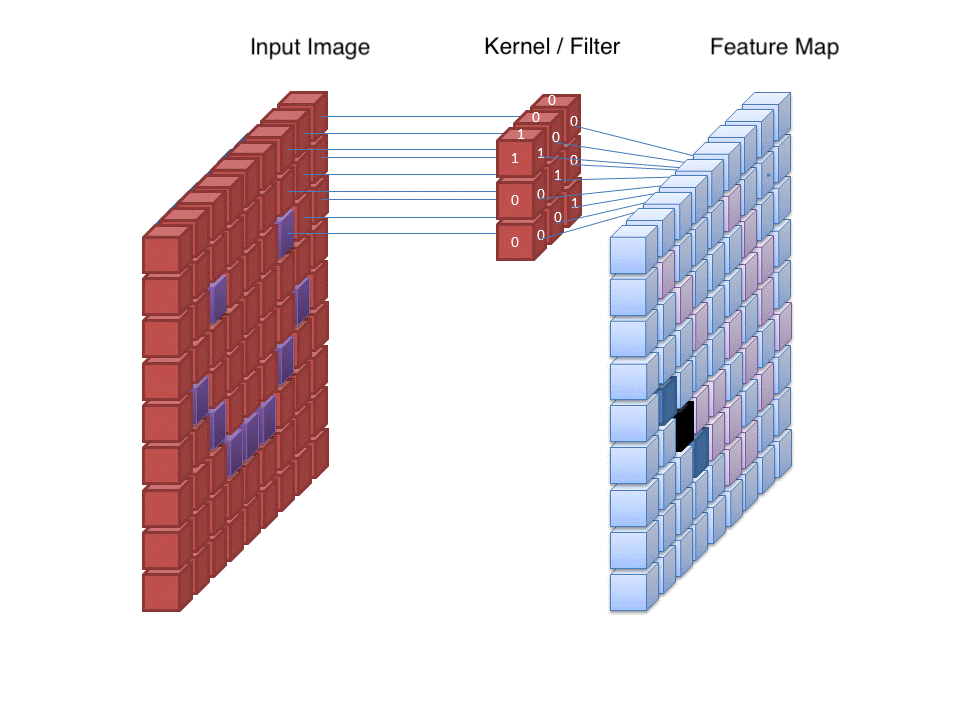
\includegraphics[width=0.5\textwidth]{images/CNN_Filter.png}
\caption[User Cecbur, \url{https://commons.wikimedia.org/wiki/File:Convolutional_Neural_Network_NeuralNetworkFilter.gif}, with labels added by Jeff Yoshimi.]{From left to right: an input image, a 3x3 convolutional filter (which detects edges with a $-45^\circ$ angle), and the resulting feature map. The filter is scanned across the image. At each stage of this scanning process, the dot product of the filtter's receptive field in the input image is computed and used to populate the feature map. This whole process is known as a convolution and a layer like this is a convolutional layer.}
\label{cnn_filter}
\end{figure}

% Receiptive field is a "patch".  
The idea is illustrated in figure \ref{cnn_filter}. A $3 \times 3$ filter is passed over a small image, from left to right and top to bottom. At each moment during this scanning process the dot product (see chapter \extref{ch_linear_algebra}) is computed between the kernel and its ``receptive field'' in the source matrix (the part of the image the filter is on top of). The product involves multiplying each weight in the filter times a corresponding in the receptive field and adding these products up. The resulting scalar is used to populate one activation in the target layer, which is called a \glossary{feature map}. In the example, the filter is an edge detector, that detects edges at a $-45^\circ$ angle, that is, edges shaped like a backslash `\textbackslash'. In the resulting feature map, notice that the highest activation is on the left side of the input image's smile. In that region the dot product of the filter with the receptive field is 2 or 3. The dot product in other parts of the image is 0 or 1. Thus the feature map shows where this kind of edge occurs in the input image.

Note that this edge detector is not programmed in. This is a neural network after all, and neural networks are trained, not programmed (section \extref{intro_comp_nn}), usually using a form of gradient descent (section \extref{sect_gradient_descent}). There is a performance advantage to these convolutional layers. All that must be trained is (in the example shown in figure \ref{cnn_filter}) $3 \times 3=9$ weights, rather than the $100 \times 100 = 10,000$ weights that would be required in a fully connected dense layer from the input layer to the feature map. This is a huge performance gain and part of what  made it possible with deep learning to train such large networks.

% This is a bit of new idea though, so think about it. It's the same template of supervised learning. The result is not a random weight matrix mapping, but a set of filters that are used to pass over an input. FOR NEXT SECTION?



\begin{figure}[h]
\centering
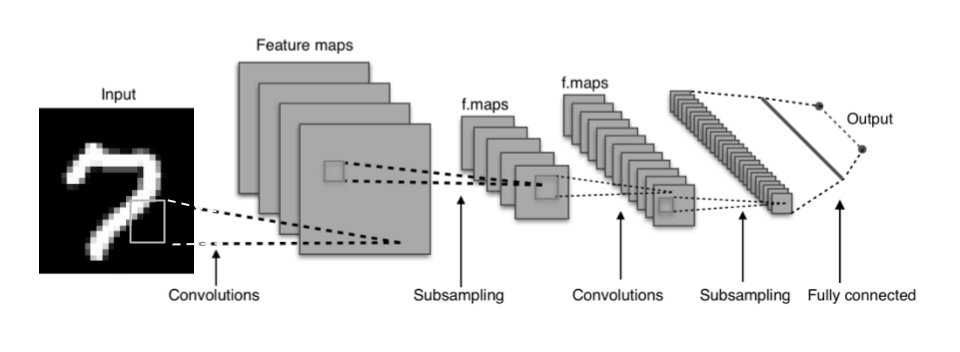
\includegraphics[scale=.45]{./images/deepNet.png}
\caption[Adapted from a creative commons image by Aphex34 at \url{https://commons.wikimedia.org/wiki/File:Typical_cnn.png} ]{A deep neural network, trained to recognize images. The convolutional layers scan over the inputs they are linked to. }
\label{deep_net2}
\end{figure}

%\begin{figure}[h]
%\centering
%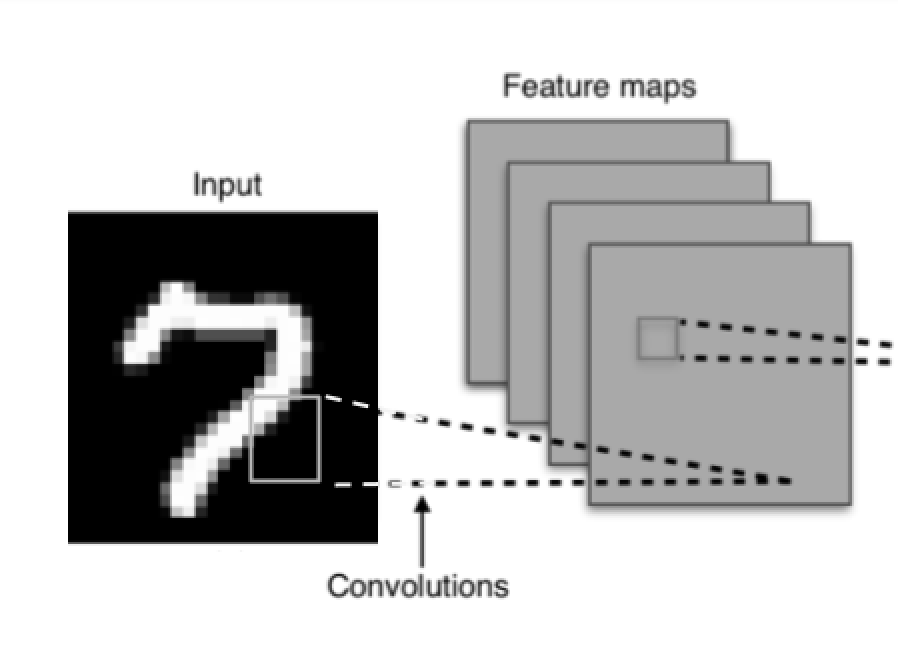
\includegraphics[scale=.4]{./images/deepNetCloseup.png}
%\caption[Closeup from a creative commons image by Aphex34 at \url{https://commons.wikimedia.org/wiki/File:Typical_cnn.png} ]{Closeup of deep neural network in chapter \extref{ch_intro} figure \extref{deep_net} showing how a set of convolutional filters like the one in \ref{cnn_filter} produce a set of feature maps. This set of feature maps is like an array of matrices, which is also known as a tensor.}
%\label{deep_net_closeup}
%\end{figure}

\section{Feature Maps and tensors}

The magic really starts to happen when we train a \emph{set of filters}, each of which produces a separate feature map.  Figure \ref{deep_net2} illustrates the idea. Note how several of the node layers say ``Feature maps'' plural, or "F.maps''. Each feature map in one of these sets is a response to a different filter, for example, edges of different orientation. This is exactly how primary visual cortex reacts to images, so this is a nice model of the brain, hence an example of computational  neuroscience. However, these networks are best known for the engineering benefits, since they are powerful pattern recognition systems.

A few things to note here.

First, a set of feature maps can be thought of as corresponding to a new kind of node layer. It is not just a  single set of nodes, but rather is itself a whole array of matrices. It's like a stack of pancakes, if each pancake is a matrix.  An array of matrices is a special kind of \glossary{tensor} (a generalization of the vectors and matrices we discussed in chapter \extref{ch_linear_algebra} to more complex numerical structures), and so computations in deep networks often involve the use of tensor mathematics.\footnote{Technically numbers and vectors and matrices are also tensors. The rank of a  tensor is the number of indices it takes to specify an ``entry'' in the tensor. A number is rank 0 because it requires no indices. Recall that a vector is like a list of numbers. A vector is rank 1 because it takes one index to specify an entry in a vector. A matrix is rank 2 because it takes two numbers to specify an entry (a row and column). A set of matrices is rank 3, because it takes 3 indices to specify an entry: one to specify a location in the array, and then a row and column index.}  

Second, these networks developing meaningful representations with training; the representations are not programmed in. This is kind of remarkable to ponder. We did not tell the network we want it to learn to respond to edges. All we focus on in training a network is inputs and outputs, using a labeled data set.  In the case shown in the figure, the training data involve images paired with numbers. The network is given nothing else but these training examples: if you see this picture, it's a 2; this picture is an 8, etc. Then the network adjusts all its parameters (all the weights in its convolutional layers), in such a way as to reduce error.  Edge detectors were learned by training, not programmed in. This is an old connectionist theme. In Nettalk (section \extref{internalRepsFF}), phonetic categories like consonant and vowel were not programmed in, but emerged with training. With simple recurrent networks  (section \extref{internalRepsRecurrent}), grammatical categories like verb and noun were not programmed in but  emerged with training.

\section{The many layers of a deep network}

In a full deep network many convolutional layers and regular ``dense'' weight layers are combined, sometimes as many as 100 or more! This allows the network to learn to identify not just simple features like edges or curves, but also \emph{features of features}, like combinations of curves which make more complex shapes, and then combinations of these shapes. 

% Improve discussion of location invariance
As can be seen in figure \ref{deep_net2}, there are other kinds of layers besides convolutional layers. Subsampling refers to methods where the size of a representation is reduced, often by scanning over the input layer, and then averaging or finding the largest value in each window (``max pooling'').  This is also called downsampling.  Also, feature maps learn to respond to specific regions of an image, it helps to have layers that are invariant to location. 

The final layers of a deep network are often more conventional fully-connected dense layers. The idea is to start with layers that learn these complex features, then to compress these representations with subsampling, and finally to present the results to the final layers, which are basically familiar backprop networks presented with the results of a whole lot of convolving and subsampling.

\section{Applications of Deep Learning}

As discussed in section \extref{deep_revolution}, deep networks and deep learning led to a revolution in neural networks beginning in the 2010s. The revolution was in engineering initially, but the history of deep networks shows that they have applications across all the domains of neural network research: engineering, computational neuroscience, and connectionism. 

They grew out of computational neuroscience models of vision in the 1970s and 1980s \cite{fukushima1982neocognitron}.  These ideas later were used to build better pattern recognition networks, an engineering application. Famous early applications included recognizing zip codes written on envelopes \cite{lecun1989backpropagation}. As deep networks became mainstream based on technical improvements (big data, GPU and hardware acceleration, better architectures and training algorithms), scientists began using them, for example, to model the response profile of neurons in the visual system (recall the discussion of figure \extref{deepLearning_Vision} in chapter \extref{ch_neuro}). 

The idea is also relevant to connectionism and computational cognitive neuroscience. You may recall from the history chapter that this idea goes  back to Oliver Selfridge and his pandemonium model, which at the time just speculated that in seeing letters a hierarchy of ``demons'' pass messages along: from edge demons to curve edges and finally to the output layer's ``B demon'' (see figure \extref{selfridge} in chapter \extref{ch_history}). These networks learn in the exact same way, but we can actually  see what their receptive fields are, and the results are sometimes strange and even disturbing.\footnote{See \url{https://distill.pub/2017/feature-visualization/} for some striking demonstrations.} 
% Work more on interpreting what is happening in that distll article, and add some material here, including pictures of the weird features. Then add some colab demos to the course.
